
\chapter{Results and Discussion}
\label{chap:results}

\section{Evaluation Metrics}
The evaluation focused on five main lens properties: sharpness, bokeh, distortion, chromatic aberration (CA), and vignetting. Sharpness was assessed using Modulation Transfer Function (MTF) charts to determine the lens's resolving power. Bokeh analysis evaluated the quality of out-of-focus areas to measure the aesthetic appeal and smoothness of the blur. Distortion measurements identified and quantified barrel and pincushion distortions using test charts. Chromatic aberration analysis examined the misalignment of RGB channels to detect and measure color fringing. Lastly, vignetting assessment measured the luminance fall-off from the center to the edges of the image to evaluate light falloff.

\section{Results}
\subsection{Successful Evaluations}

\subsubsection{Vignetting}
\begin{table}[H]
    \centering
    \caption{Vignetting Assessment Results}
    \label{tab:vignetting_results}
    \resizebox{\textwidth}{!}{%
    \begin{tabular}{|c|c|c|}
        \hline
        \textbf{Photo ID} & vignette\_20241215\_132956\_2J9B3461.CR2 & vignette\_20241215\_140626\_2J9B3465.CR2 \\ \hline
        \textbf{Center Intensity} & 68.26 & 65.29 \\ \hline
        \textbf{Top Left} & 41.27 & 38.81 \\ \hline
        \textbf{Top Right} & 34.51 & 32.51 \\ \hline
        \textbf{Bottom Left} & 26.87 & 25.26 \\ \hline
        \textbf{Bottom Right} & 19.86 & 17.09 \\ \hline
    \end{tabular}%
    }
\end{table}

\begin{figure}[H]
    \centering
    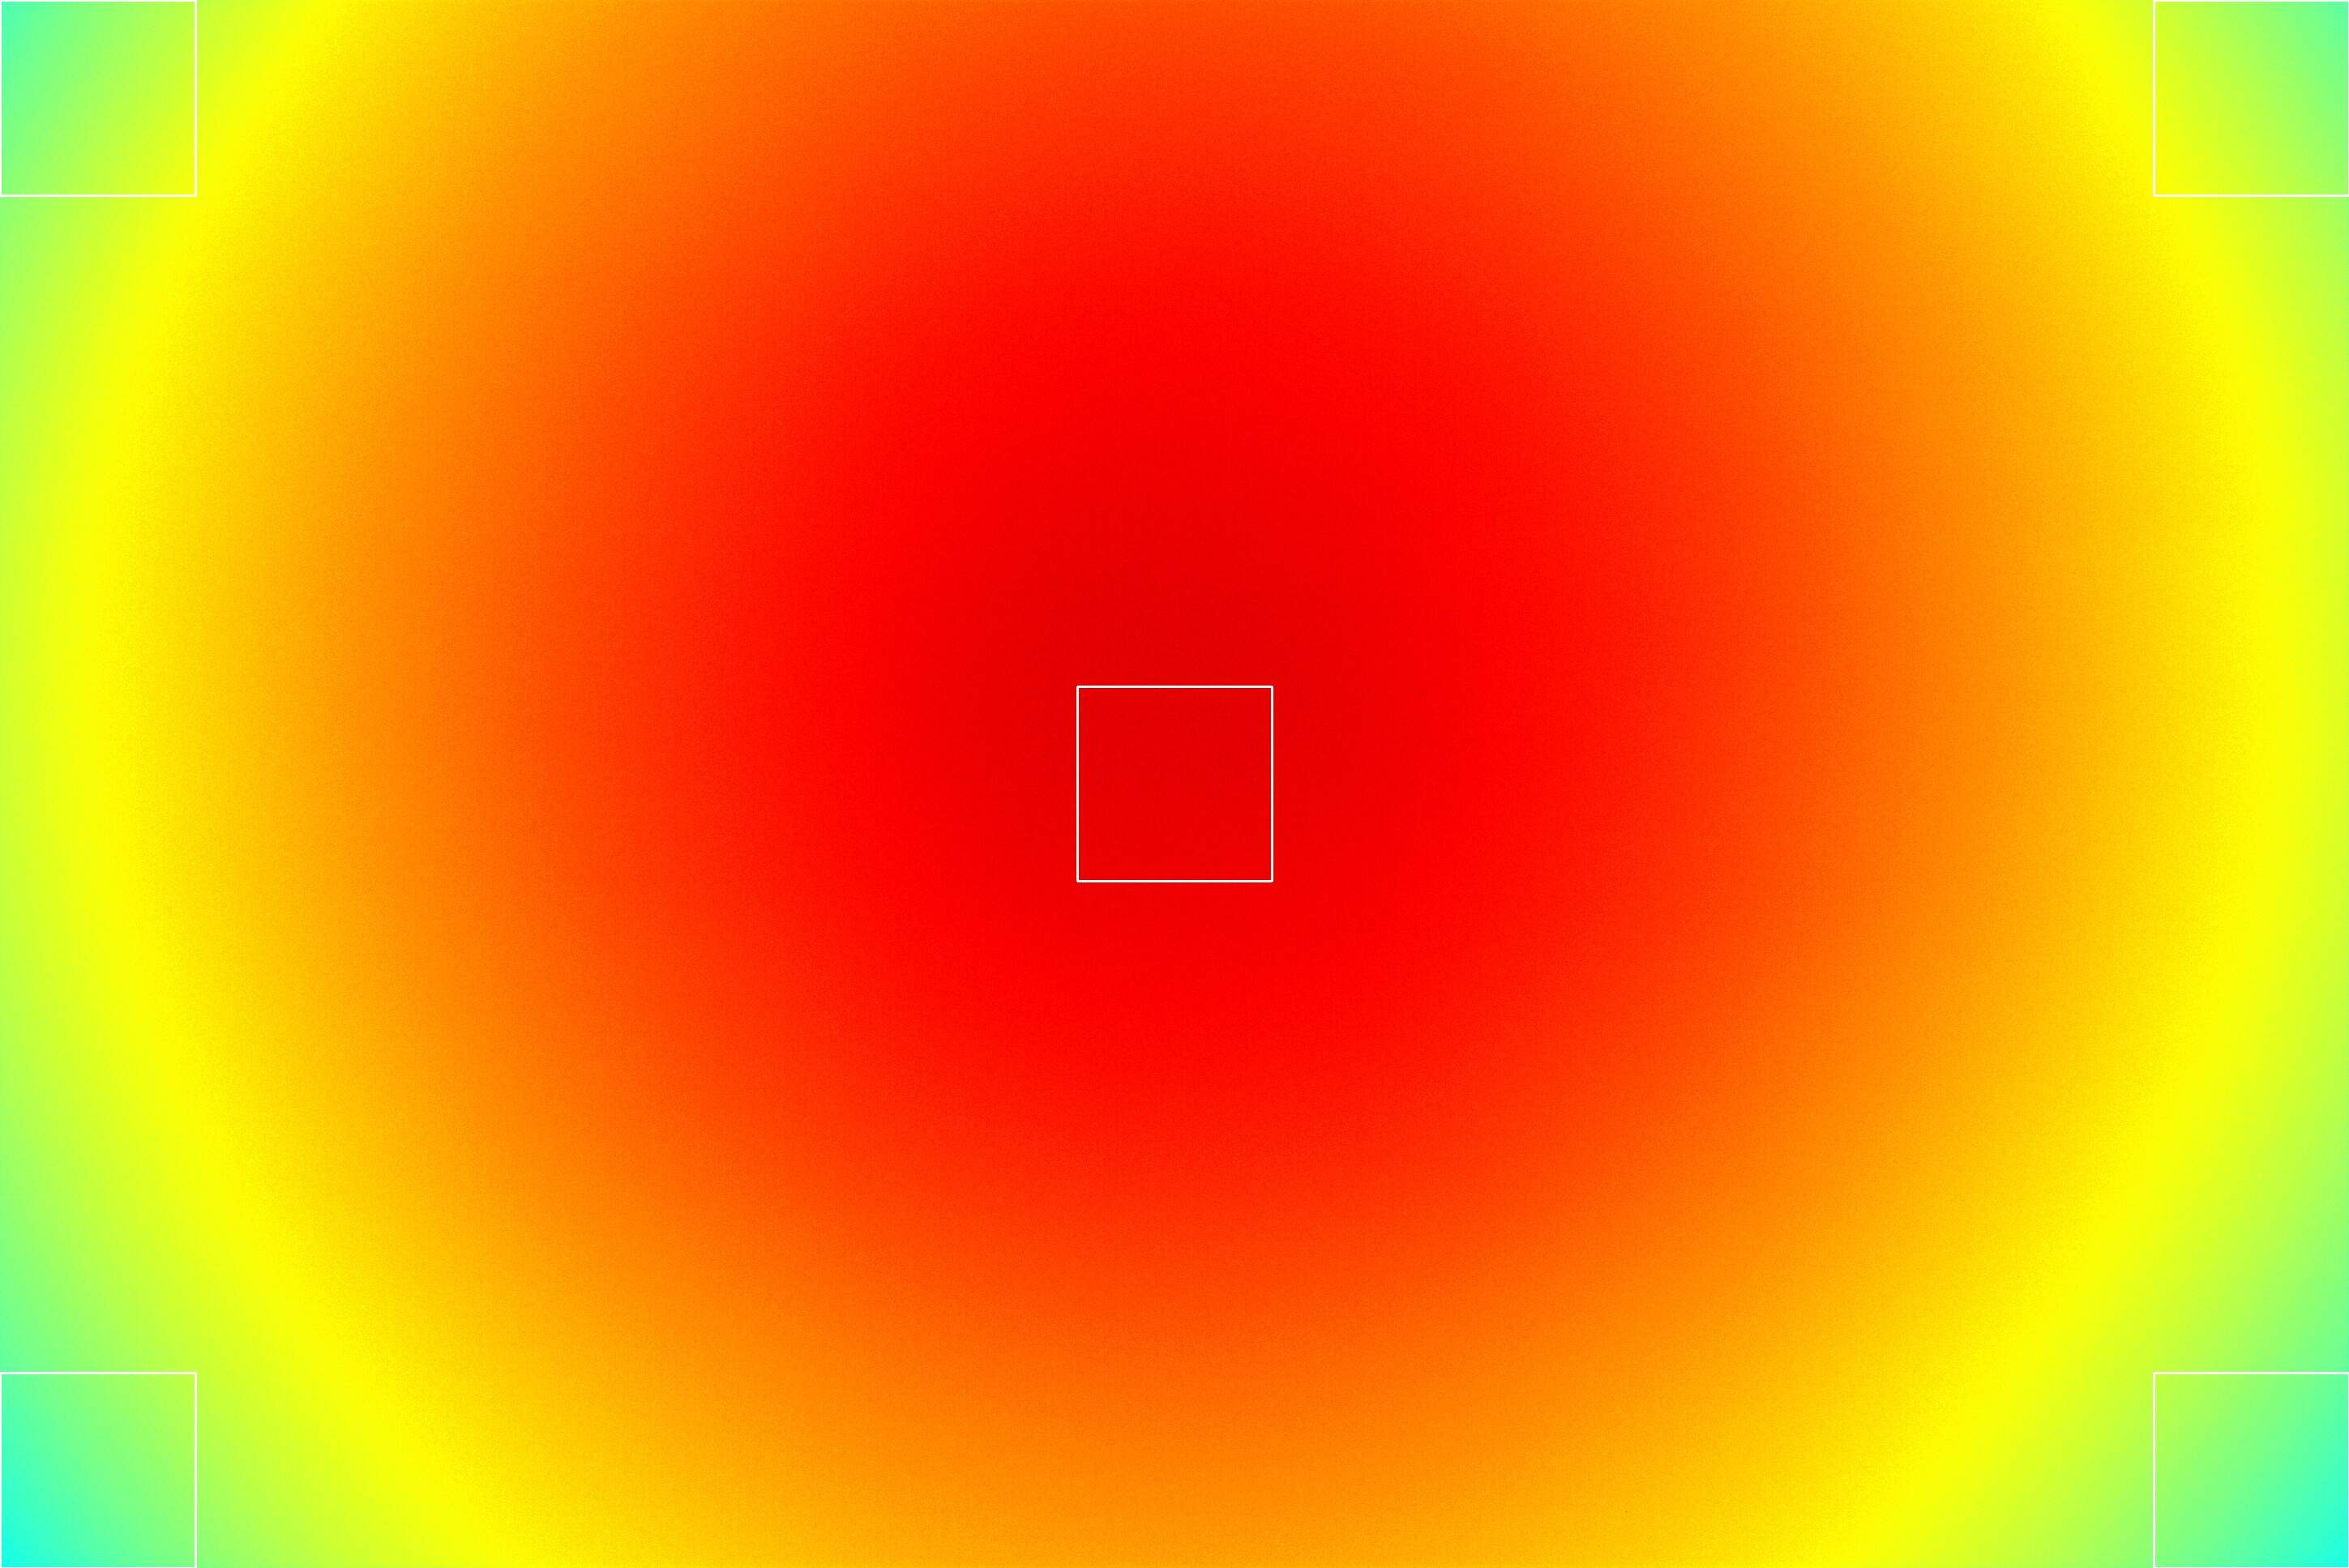
\includegraphics[width=0.8\textwidth]{Images/vignette_analysis_20241209_135329.jpg}
    \caption{Vignetting Analysis Visualization}
    \label{fig:vignetting_visualization}
\end{figure}

The vignetting scores indicated a noticeable luminance fall-off, which is expected under wide aperture settings. The consistent reduction in intensity from the center to the corners validates the application's accuracy in this metric.

\subsubsection{Bokeh}
\begin{table}[H]
    \centering
    \caption{Bokeh Assessment Scores}
    \label{tab:bokeh_scores}
    \resizebox{\textwidth}{!}{%
    \begin{tabular}{|c|c|}
        \hline
        \textbf{Photo ID} & bokeh\_20241215\_141412\_2J9B3466.CR2 \\ \hline
        \textbf{Overall Score} & 66.79 \\ \hline
        \textbf{Shape Regularity} & 44.48 \\ \hline
        \textbf{Color Fringing} & 90.81 \\ \hline
    \end{tabular}%
    }
\end{table}


\begin{figure}[H]
    \centering
    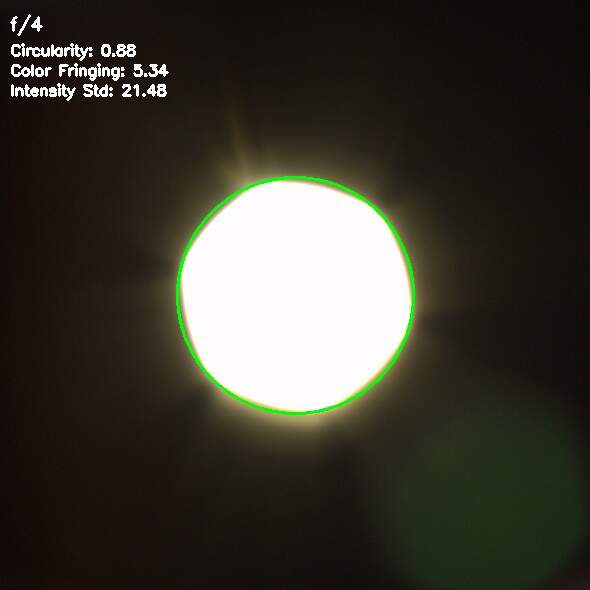
\includegraphics[width=0.7\textwidth]{Images/bokeh_analysis_20241212_234642.jpg}
    \caption{Bokeh Analysis Visualization}
    \label{fig:bokeh_visualization}
\end{figure}

The bokeh scores reflected the smoothness and aesthetic quality of the out-of-focus areas. High scores in color fringing indicate minimal color distortions, contributing to pleasing bokeh effects.

\subsection{Partial or Unsuccessful Evaluations}

\subsubsection{Sharpness}
\begin{table}[H]
    \centering
    \caption{Sharpness Assessment Scores}
    \label{tab:sharpness_scores}
    \resizebox{\textwidth}{!}{%
    \begin{tabular}{|c|c|}
        \hline
        \textbf{Photo ID} & sharpness\_20241215\_152555\_2J9B3467.CR2 \\ \hline
        \textbf{Sharpness Score} & 3.26 \\ \hline
        \textbf{Traditional Score} & 3.80 \\ \hline
        \textbf{SIFT Score} & 1.98 \\ \hline
    \end{tabular}%
    }
\end{table}

\begin{figure}[H]
    \centering
    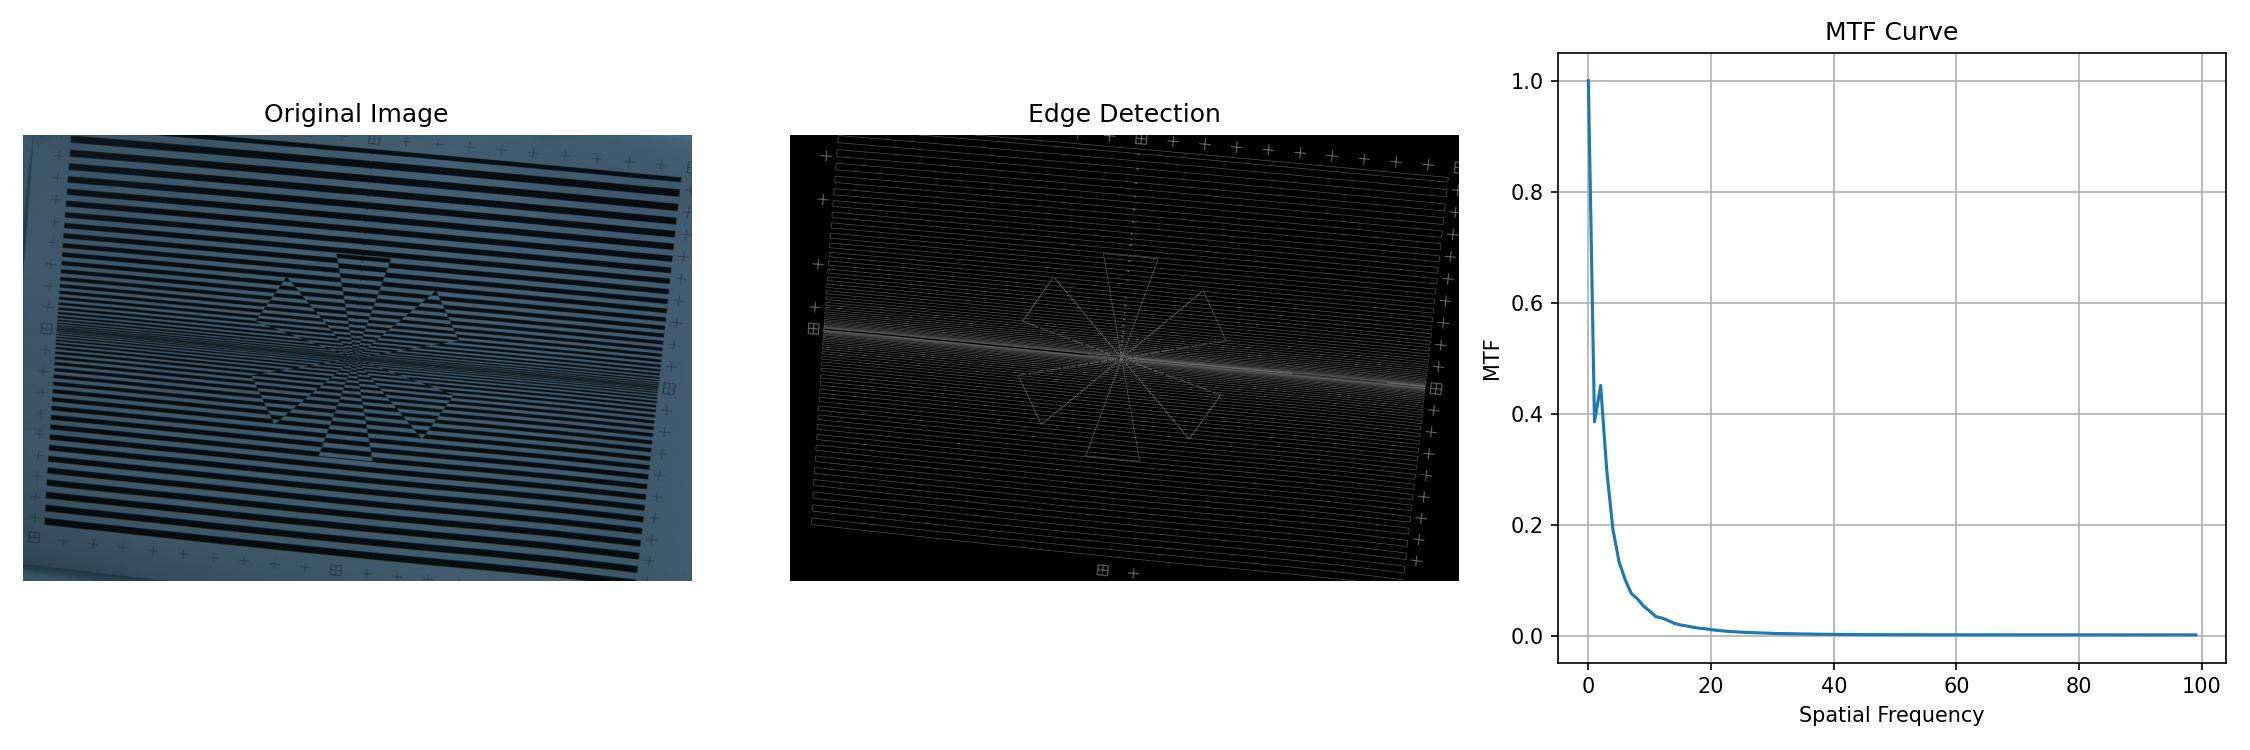
\includegraphics[width=0.8\textwidth]{Images/sharpness_analysis_20241211_224531.jpg}
    \caption{Sharpness Analysis Visualization}
    \label{fig:sharpness_analysis}
\end{figure}

While the application attempted to measure the lens's resolving power, the results were inconsistent. Some lenses showed expected sharpness levels, but overall, the sharpness measurements did not consistently align with theoretical benchmarks or visual assessments.

\subsubsection{Chromatic Aberration (CA)}
\begin{table}[H]
    \centering
    \caption{Chromatic Aberration Assessment Scores}
    \label{tab:ca_scores}
    \resizebox{\textwidth}{!}{%
    \begin{tabular}{|c|c|c|c|}
        \hline
        \textbf{Photo ID} & chromatic\_20241215\_161105\_sharpness\_f4\_20241211\_212111.CR2 \\ \hline
        \textbf{Chromatic Aberration Score} & 34.72 \\ \hline
        \textbf{Lateral CA} & R-G: 3.89, R-B: 1.16, G-B: 4.98 \\ \hline
        \textbf{Longitudinal CA} & R-G: 1.21, R-B: 1.71, G-B: 1.41 \\ \hline
    \end{tabular}%
    }
\end{table}



\begin{figure}[H]
    \centering
    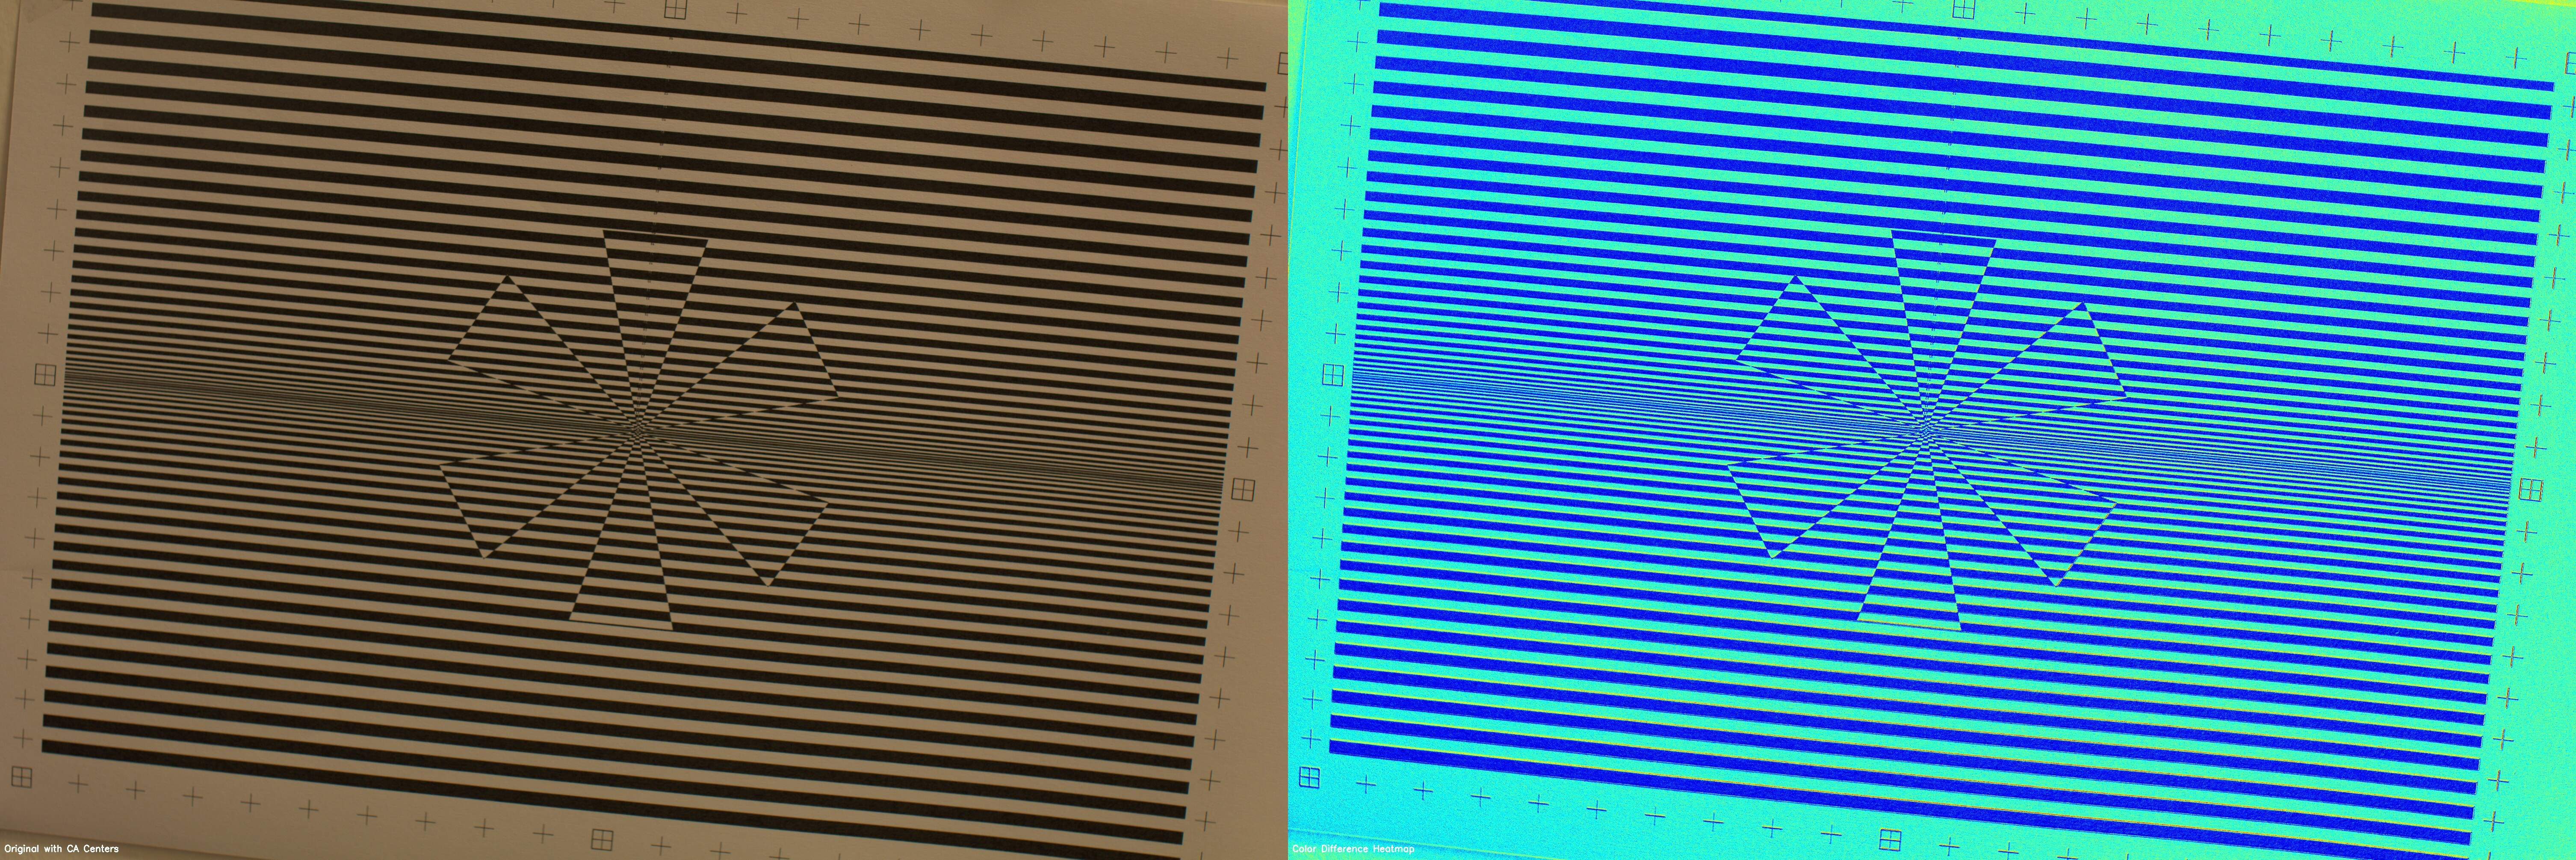
\includegraphics[width=1\textwidth]{Images/ca_analysis_20241211_234543.jpg}
    \caption{Chromatic Aberration Analysis Visualization }
    \label{fig:ca_visualization}
\end{figure}

The CA scores indicate moderate color fringing, but the measurements lacked consistency across different photos. Factors such as high ISO settings and image noise may have contributed to unreliable CA assessments.

\subsubsection{Distortion}
\begin{table}[H]
    \centering
    \caption{Distortion Assessment Scores}
    \label{tab:distortion_scores}
    \resizebox{\textwidth}{!}{%
    \begin{tabular}{|c|c|}
        \hline
        \textbf{Photo ID} & distortion\_20241215\_161602\_sharpness\_f4\_20241211\_212111.CR2 \\ \hline
        \textbf{Mean Deviation} & 2.20 \\ \hline
        \textbf{Max Deviation} & 3.17 \\ \hline
    \end{tabular}%
    }
\end{table}

The distortion analysis identified pincushion distortion; however, the accuracy of these measurements was questionable due to potential alignment issues and high image noise.

Despite these challenges, the application succeeded in visualizing all intended lens properties, providing valuable insights even when quantitative measurements were inconsistent.

\section{Testing Methodology Validation}

\subsection{Repeatability Testing}
Testing focused on result consistency across different scenarios. Basic repeatability was verified through identical test conditions (same camera, lens, settings, and scenario), which produced consistent results with negligible variations from sensor noise. This established a baseline for measurement reliability.

\subsection{Environmental Adaptability}
Multiple captures with slight ambient lighting variations demonstrated the system's robustness. Results remained within acceptable error margins despite environmental fluctuations, validating the lighting compensation mechanisms.

\subsection{Cross-Platform Performance}
Testing examined lens behavior across different camera bodies:

\subsubsection{Same-Generation Bodies}
Comparing two Canon EOS 5D Mark III bodies (shutter counts ~100,000 vs ~260,000) revealed consistent measurements, indicating result stability across different units of the same model.

\subsubsection{Different Sensor Formats}
Tests between full-frame (5D Mark III) and crop-sensor bodies (80D) showed expected variations in field of view while maintaining consistent sharpness measurements when accounting for sensor differences.

\subsubsection{Cross-Brand Adaptation}
Nikon lenses (18-55mm f/3.5-5.6G, 50mm f/1.8) were tested on both native (D3400) and adapted (Canon 80D) bodies using the Novoflex adapter. Results showed minimal impact on optical performance, though autofocus capabilities were affected.

\subsection{Zoom Lens Characteristics}
Analysis of zoom lenses revealed variations in sharpness across focal lengths, providing insights into optimal shooting ranges for each lens. This testing validated the system's ability to track performance changes through a lens's zoom range.

\section{Limitations}
Several limitations impacted the accuracy and reliability of the lens evaluations:

\begin{itemize}
    \item \textbf{Image Noise}: A significant amount of noise was present in the images used for evaluation. This noise interfered with the application's ability to accurately measure and quantify lens properties, particularly affecting sharpness and chromatic aberration assessments.
    \item \textbf{Pixel Scale}: The pixel scale used in the analysis was excessively large, leading to confusion and difficulties in interpreting the quantitative data. This issue hindered precise measurements and contributed to inconsistencies in evaluating certain lens properties.
    \item \textbf{Environmental Factors}: Uneven lighting conditions and slight misalignments of test charts introduced variability in the results. These factors compromised the consistency of measurements, especially for metrics sensitive to lighting and alignment.
\end{itemize}

These limitations highlight the need for improved image acquisition protocols and enhanced processing algorithms to mitigate noise and optimize pixel scaling.

\section{Comparative Analysis}
Direct comparison with industry tools like Imatest and DxOMark proved unfeasible due to licensing restrictions and commercial access limitations. Imatest's commercial licensing model and DxOMark's proprietary testing methodology was one of the reasons of not including side-by-side result validation. The project timeline also constrained the scope for extensive comparative testing. Future work could explore partnerships with commercial testing facilities to enable proper benchmarking of the application's accuracy and reliability against these established tools.

\section{Discussion}
The evaluation metrics revealed that the application possesses strengths in assessing certain lens properties while encountering challenges with others. Specifically, the successful measurement of vignetting and bokeh demonstrates the tool's potential in providing valuable insights into lens performance. The ability to visualize these properties effectively supports photographers in making informed decisions about lens quality.

However, the inconsistent results in sharpness and chromatic aberration assessments indicate areas for improvement. The presence of significant image noise and an overly large pixel scale adversely affected the application's performance in these metrics. Addressing these issues through enhanced image preprocessing and calibration techniques is essential for improving measurement accuracy.

The partial success in distortion measurements suggests that the application requires further refinement in detecting and quantifying geometric distortions. Implementing more robust algorithms and optimizing test chart alignment procedures could enhance the reliability of distortion assessments.

\subsection{Strengths}
\begin{itemize}
    \item \textbf{Vignetting Measurement}: The application accurately quantified luminance fall-off, providing reliable data that aligns with theoretical expectations.
    \item \textbf{Bokeh Analysis}: Successfully evaluated the aesthetic quality of out-of-focus areas, offering objective scores that correlate with subjective assessments.
    \item \textbf{Visualization Capabilities}: Managed to visualize all intended lens properties, facilitating a better understanding of lens performance despite quantitative inconsistencies.
\end{itemize}

\subsection{Weaknesses}
\begin{itemize}
    \item \textbf{Sharpness Assessment}: Inconsistent measurements due to high image noise and large pixel scales compromised the reliability of sharpness scores.
    \item \textbf{Chromatic Aberration Detection}: Partial success in identifying color fringing suggests the need for more refined detection algorithms.
    \item \textbf{Distortion Quantification}: Limited effectiveness in accurately measuring geometric distortions indicates the necessity for improved analysis methods.
\end{itemize}

\subsection{Recommendations for Improvement}
To enhance the application's performance, the following improvements are recommended:

\begin{itemize}
    \item \textbf{Noise Reduction}: Implement advanced image preprocessing techniques to minimize noise and enhance measurement accuracy.
    \item \textbf{Pixel Scaling Optimization}: Adjust the pixel scale to a more manageable size to facilitate clearer data interpretation.
    \item \textbf{Algorithm Enhancement}: Refine existing algorithms or develop new ones to improve the detection and quantification of sharpness, chromatic aberration, and distortion.
    \item \textbf{Environmental Controls}: Standardize image acquisition conditions to reduce variability caused by uneven lighting and misaligned test charts.
\end{itemize}

\chapter{Conclusion and Further Work}

\section{Summary of Findings}
This thesis presented the development of a Python application for evaluating lens properties. The application successfully captured and analyzed images to assess various lens properties, providing a comprehensive score for each property. Notably, the application accurately measured vignetting and bokeh, aligning with theoretical expectations and subjective assessments.

The methodology includes support for RAW image capture, parameterized batch processing, and integration of standardized test charts. A web-based user interface, developed with NiceGUI, enhances usability and supports diverse use cases for beginners and professionals alike.

The research explores fundamental aspects of lens performance, including sharpness, chromatic aberrations, geometric distortions, vignetting, bokeh, and dynamic range. It also examines the challenges posed by metadata reliability and camera control standardization. Robust error handling and recovery mechanisms are implemented to ensure system stability.

\section{Limitations}
The application is currently limited to cameras that are compatible with the Python libraries utilized in its implementation, particularly gphoto2 used to access the camera \cite{gphoto2_compatible}. This dependency on library support restricts the system’s compatibility to a subset of cameras, potentially excluding certain models or brands. The compatibility is further narrowed by different implementations of different manufacturers protocols.

Lighting conditions significantly impact lens evaluation by affecting the accuracy and consistency of results. Variations in intensity, color temperature, and uniformity can influence the measurements of various lens properties. Furthermore, achieving even illumination, especially for test charts, often requires specialized setups that may not always be accessible for at-home lens testing.

The reliance on EXIF metadata for extracting camera and lens information presents challenges due to inconsistent implementation across manufacturers and the lack of a formal standard. This makes metadata an unreliable sole source of information.

High-resolution RAW image analysis and advanced processing algorithms might place significant computational demands on lower-end hardware, potentially affecting performance.

\section{Future Work}

Future research could explore the integration of motorized testing setups to achieve greater precision in measurements. Additionally, expanding the application to support a wider range of camera models and lenses would enhance its versatility. Developing more sophisticated algorithms to reduce image noise and optimize pixel scaling could further improve the accuracy of sharpness and chromatic aberration assessments. Creating an extensive catalog of lens evaluations would provide a valuable reference for photographers and technicians, providing informed decision-making in lens selection.

